% This LaTeX was auto-generated from MATLAB code.
% To make changes, update the MATLAB code and export to LaTeX again.

\documentclass{article}

\usepackage[utf8]{inputenc}
\usepackage[T1]{fontenc}
\usepackage{lmodern}
\usepackage{graphicx}
\usepackage{color}
\usepackage{listings}
\usepackage{hyperref}
\usepackage{amsmath}
\usepackage{amsfonts}
\usepackage{epstopdf}
\usepackage{matlab}

\sloppy
\epstopdfsetup{outdir=./}
\graphicspath{ {./ejercicio02_images/} }

\begin{document}

\matlabtitle{Ejercicio Nº2}


\begin{matlabcode}
clear;clc;
\end{matlabcode}

\begin{par}
\begin{flushleft}
Se definen simbólicas las variables
\end{flushleft}
\end{par}

\begin{matlabcode}
syms t vc(t) il(t) C L R1 R2 E;
\end{matlabcode}

\begin{par}
\begin{flushleft}
Se plantean las ecuaciones y se obtienen las matrices de la forma generalizada
\end{flushleft}
\end{par}

\begin{matlabcode}
M=[-C 0;0 L]
\end{matlabcode}
\begin{matlabsymbolicoutput}
M = 
    $\displaystyle \left(\begin{array}{cc}
-C & 0\\
0 & L
\end{array}\right)$
\end{matlabsymbolicoutput}
\begin{matlabcode}
N=[-1/R1 -1;-1 R2]
\end{matlabcode}
\begin{matlabsymbolicoutput}
N = 
    $\displaystyle \left(\begin{array}{cc}
-\frac{1}{R_1 } & -1\\
-1 & R_2 
\end{array}\right)$
\end{matlabsymbolicoutput}
\begin{matlabcode}
u=[-E/R1;0]
\end{matlabcode}
\begin{matlabsymbolicoutput}
u = 
    $\displaystyle \left(\begin{array}{c}
-\frac{\textrm{E}}{R_1 }\\
0
\end{array}\right)$
\end{matlabsymbolicoutput}

\begin{par}
\begin{flushleft}
Se expresan las matrices de la forma normalizada
\end{flushleft}
\end{par}

\vspace{1em}

\begin{matlabcode}
A=-1.*(M\N)
\end{matlabcode}
\begin{matlabsymbolicoutput}
A = 
    $\displaystyle \left(\begin{array}{cc}
-\frac{1}{C R_1 } & -\frac{1}{C}\\
\frac{1}{L} & -\frac{R_2 }{L}
\end{array}\right)$
\end{matlabsymbolicoutput}
\begin{matlabcode}

B=M\u
\end{matlabcode}
\begin{matlabsymbolicoutput}
B = 
    $\displaystyle \left(\begin{array}{c}
\frac{\textrm{E}}{C R_1 }\\
0
\end{array}\right)$
\end{matlabsymbolicoutput}

\begin{par}
\begin{flushleft}
Se definen las variables de estado
\end{flushleft}
\end{par}

\begin{matlabcode}
x=[vc;il]
\end{matlabcode}
\begin{matlabsymbolicoutput}
x(t) = 
    $\displaystyle \left(\begin{array}{c}
\textrm{vc}\left(t\right)\\
\textrm{il}\left(t\right)
\end{array}\right)$
\end{matlabsymbolicoutput}

\begin{par}
\begin{flushleft}
Expresando el sistema en forma diferencial
\end{flushleft}
\end{par}

\begin{matlabcode}
odes = diff(x) ==  A*x + B
\end{matlabcode}
\begin{matlabsymbolicoutput}
odes(t) = 
    $\displaystyle \left(\begin{array}{c}
\frac{\partial }{\partial t}\;\textrm{vc}\left(t\right)=\frac{\textrm{E}}{C R_1 }-\frac{\textrm{vc}\left(t\right)}{C R_1 }-\frac{\textrm{il}\left(t\right)}{C}\\
\frac{\partial }{\partial t}\;\textrm{il}\left(t\right)=\frac{\textrm{vc}\left(t\right)}{L}-\frac{R_2  \textrm{il}\left(t\right)}{L}
\end{array}\right)$
\end{matlabsymbolicoutput}

\begin{par}
\begin{flushleft}
Resolviendo el sistema con el comando dsolve
\end{flushleft}
\end{par}

\begin{matlabcode}
[vSol(t), iSol(t)] = dsolve(odes);
\end{matlabcode}

\begin{par}
\begin{flushleft}
\textbf{Tensión del capacitor}
\end{flushleft}
\end{par}

\begin{matlabcode}
vSol(t) = simplify(vSol(t))
\end{matlabcode}
\begin{matlabsymbolicoutput}
vSol(t) = 
    $\displaystyle \begin{array}{l}
\frac{e^{-\sigma_1 }  {\left(\textrm{E} e^{\sigma_1 } +C_{23}  R_1 +C_{23}  R_2 +C_{24}  R_1  \sigma_2 +C_{24}  R_2  \sigma_2 \right)}}{R_1 +R_2 }\\
\mathrm{}\\
\textrm{where}\\
\mathrm{}\\
\;\;\sigma_1 =\frac{t {\left(L+\sqrt{C^2  {R_1 }^2  {R_2 }^2 -4 C L {R_1 }^2 -2 C L R_1  R_2 +L^2 }+C R_1  R_2 \right)}}{2 C L R_1 }\\
\mathrm{}\\
\;\;\sigma_2 =e^{\frac{t \sqrt{C^2  {R_1 }^2  {R_2 }^2 -4 C L {R_1 }^2 -2 C L R_1  R_2 +L^2 }}{C L R_1 }} 
\end{array}$
\end{matlabsymbolicoutput}

\begin{par}
\begin{flushleft}
\textbf{Corriente del inductor}
\end{flushleft}
\end{par}

\begin{matlabcode}
iSol(t) = simplify(iSol(t))
\end{matlabcode}
\begin{matlabsymbolicoutput}
iSol(t) = 
    $\displaystyle \begin{array}{l}
e^{-\frac{t \sigma_4 }{2 C L R_1 }}  {\left(R_2 -\frac{\sigma_4 }{2 C R_1 }\right)} {\left(C_{23} -\frac{2 C \textrm{E} L R_1  \sigma_1  e^{\sigma_5 }  \sigma_2 }{\sigma_4  \sigma_6 }\right)}+e^{-\frac{t \sigma_3 }{2 C L R_1 }}  {\left(R_2 -\frac{\sigma_3 }{2 C R_1 }\right)} {\left(C_{24} +\frac{2 C \textrm{E} L R_1  \sigma_1  e^{-\sigma_5 }  \sigma_2 }{\sigma_3  \sigma_6 }\right)}\\
\mathrm{}\\
\textrm{where}\\
\mathrm{}\\
\;\;\sigma_1 =e^{\frac{R_2  t}{2 L}} \\
\mathrm{}\\
\;\;\sigma_2 =e^{\frac{t}{2 C R_1 }} \\
\mathrm{}\\
\;\;\sigma_3 =L-\sigma_6 +C R_1  R_2 \\
\mathrm{}\\
\;\;\sigma_4 =L+\sigma_6 +C R_1  R_2 \\
\mathrm{}\\
\;\;\sigma_5 =\frac{t \sigma_6 }{2 C L R_1 }\\
\mathrm{}\\
\;\;\sigma_6 =\sqrt{C^2  {R_1 }^2  {R_2 }^2 -4 C L {R_1 }^2 -2 C L R_1  R_2 +L^2 }
\end{array}$
\end{matlabsymbolicoutput}

\begin{par}
\begin{flushleft}
Reemplazando los valores de E,R1, R2, L y C
\end{flushleft}
\end{par}

\begin{matlabcode}
clear C L R1 R2 E;
syms C1 C2;
R1=1;R2=1;L=1;C=1;E=1;
A=subs(A);
B=subs(B);
\end{matlabcode}

\matlabheading{Autovalores del circuito}

\begin{matlabcode}
autovalores= eig(A)
\end{matlabcode}
\begin{matlabsymbolicoutput}
autovalores = 
    $\displaystyle \left(\begin{array}{c}
-1-i\\
-1+i
\end{array}\right)$
\end{matlabsymbolicoutput}

\begin{par}
\begin{flushleft}
Las ecuaciones diferenciales son
\end{flushleft}
\end{par}

\begin{matlabcode}
odes = diff(x) == A*x + B
\end{matlabcode}
\begin{matlabsymbolicoutput}
odes(t) = 
    $\displaystyle \left(\begin{array}{c}
\frac{\partial }{\partial t}\;\textrm{vc}\left(t\right)=1-\textrm{vc}\left(t\right)-\textrm{il}\left(t\right)\\
\frac{\partial }{\partial t}\;\textrm{il}\left(t\right)=\textrm{vc}\left(t\right)-\textrm{il}\left(t\right)
\end{array}\right)$
\end{matlabsymbolicoutput}

\matlabheading{Estableciendo condiciones iniciales y tiempo de simulación}

\begin{par}
\begin{flushleft}
Para el primer par de condiciones iniciales
\end{flushleft}
\end{par}

\begin{matlabcode}
v0=1;
i0=1;
ti=0;
tf=4*pi;
Xant=[v0;i0];
constantes=x(0)==Xant;
[vSol(t), iSol(t)] = dsolve(odes,constantes)
\end{matlabcode}
\begin{matlabsymbolicoutput}
vSol(t) = 
    $\displaystyle \frac{e^{-t}  \cos \left(t\right)}{2}+\frac{e^{-t}  \sin \left(t\right)}{2}+\frac{1}{2}$
iSol(t) = 
    $\displaystyle \frac{e^{-t}  \cos \left(t\right)}{2}-\frac{e^{-t}  \sin \left(t\right)}{2}+\frac{1}{2}$
\end{matlabsymbolicoutput}


\begin{par}
\begin{flushleft}
Para el segundo par de condiciones iniciales
\end{flushleft}
\end{par}

\begin{matlabcode}
clear t;
syms t;
v0=-1;
i0=-1;
ti=0;
tf=4*pi;
Xant=[v0;i0];
constantes=x(0)==Xant;
[v2Sol(t), i2Sol(t)] = dsolve(odes,constantes)
\end{matlabcode}
\begin{matlabsymbolicoutput}
v2Sol(t) = 
    $\displaystyle \frac{1}{2}-\frac{3 e^{-t}  \sin \left(t\right)}{2}-\frac{3 e^{-t}  \cos \left(t\right)}{2}$
i2Sol(t) = 
    $\displaystyle \frac{3 e^{-t}  \sin \left(t\right)}{2}-\frac{3 e^{-t}  \cos \left(t\right)}{2}+\frac{1}{2}$
\end{matlabsymbolicoutput}

\begin{par}
\begin{flushleft}
Gráfico de las soluciones
\end{flushleft}
\end{par}

\begin{matlabcode}
h=0.1;
t=ti:h:tf;
b=plot(i2Sol(t),v2Sol(t),'-b',iSol(t),vSol(t),'-r');
title('Phase portrait')
xlabel('Corriente en el inductor [A]')
ylabel('Voltaje en el capacitor [V]')
grid on
legend({'[vo=1;io=10]','[vo=1;i0=1]'})
xlim([-1.00 1.00])
ylim([-1.00 1.00])
\end{matlabcode}
\begin{center}
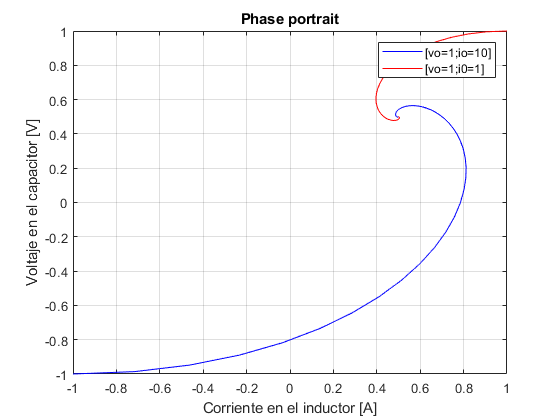
\includegraphics[width=\maxwidth{56.196688409433015em}]{figure_0_01}
\end{center}

\end{document}
